%% V1.0
%% by Gabriel Garcia, gabrcg@gmail.com
%% This is a template for Udacity projects using IEEEtran.cls

%% Be Udacious!

\documentclass[10pt,journal,compsoc]{IEEEtran}

\usepackage[pdftex]{graphicx}    
\usepackage{cite}
\hyphenation{op-tical net-works semi-conduc-tor}


\begin{document}

\title{Udacity RoboND Project: Where Am I? \\
    \huge Adaptive Monte-Carlo Localization}

\author{Trijeet Modak}

\markboth{Localization project, Robotics Nanodegree Program, Udacity}%
{}
\IEEEtitleabstractindextext{%

\begin{abstract}
This paper aims to localize custom robots using ROS's Adaptive Monte-Carlo Localization (AMCL) package in a simulated environment of Gazebo/RViz. Two mobile robots are designed, each with unique wheel and chassis properties and equipped with a camera and a laser rangefinder. On proper tuning of the robot's configuration parameters, the robots localized themselves accurately, navigated autonomously and reached the defined goal on the map.
\end{abstract}

% Note that keywords are not normally used for peerreview papers.
\begin{IEEEkeywords}
Robot, Localization, Udacity.
\end{IEEEkeywords}}


\maketitle
\IEEEdisplaynontitleabstractindextext
\IEEEpeerreviewmaketitle
\section{Introduction}
\label{sec:introduction}

\IEEEPARstart{I}{t} is quite intuitive that a mobile robot, capable of autonomous navigation, must know its current location in its operating environment. Thus before taking any step ahead, a robot must estimate its location with high accuracy, failing which it may lead to severe damages both to itself and to life and/or property in its vicinity. In robotics, the problem of approximation of a robot's location in its operating environment is termed as $Robot$  $Localization$ or simply $Localization$. 

The objective of this project is to accurately localize two individual mobile robots in a simulation environment such that they are able to autonomously navigate towards a predefined goal on a given map.

\section{Background / Formulation}
There are a number of approaches through which $Localization$ may be achieved for a mobile robot. The most popular algorithms used for localization include Markov\cite{}fox1999markov localization, Grid based\cite{vu2008grid} localization, Kalman Filter based\cite{chen2015fusion} localization and Monte-Carlo\cite{fox1999monte}\cite{dellaert1999monte} localization. Kalman Filter and Monte-Carlo (also known as Particle Filter) based localization are often used for their high accuracy and lesser susceptibility to noise. and are discussed below.

\subsection{Kalman Filter}
The Kalman Filter (KF) is an estimation algorithm and is widely used in control systems, especially where the sensor measurements are noisy or has a considerable degree of uncertainty. It is fast, efficient, and can make an accurate estimate even with sparse data. Since its success with the Apollo program, the Kalman filter has become one of the most practical algorithms in the field of controls engineering.

The algorithm starts with an initial guess of the system's current state and iterates over following two steps continuously.
\begin{enumerate}
    \item Measurement Update: sensor measurements are collected to update the current state of the system.
    \item State Prediction: future state of the system is predicted using the current state obtained above.
\end{enumerate}
After a few iterations, the estimates converge to an accurate value.

The standard KF algorithm can only be applied to linear systems, where the output is proportional to the input. Since most real-world systems, such as robotics, are non-linear in nature, a variation of KF, known as the Extended Kalman Filter (EKF) algorithm, is more appropriate in such applications. Another variation of the standard KF, called Unscented Kalman Filter (UKF) is used in systems which are extremely non-linear.


\subsection{Monte-Carlo Localization}
Monte-Carlo Localization (MCL) is arguably the most widely used localization algorithm in robotic applications, especially to keep track of a robot's position even when its initial position is unknown. Virtual elements called particles are used to localize a robot. Each particle represents the robot's probable (hypothesized) location and orientation (collectively called the robot's pose) in the operating environment. Each particle is assigned an weight that determines the importance of the particle with respect to its accuracy in representing the robot's pose. 

The algorithm too is a two step process, iterated over and over again, where each iteration outputs a pose estimate of the current robot state. Initially the particles are randomly and uniformly distributed throughout the entire map. In the first step, the hypothetical state is computed as the robot moves and the weights of the particles are computed using the latest sensor readings. The motion and measurements are added to the previous state. In the second step, the particles are re-sampled in which only those particles that have a significant weight (the new pose estimates) are carried forward to the next iteration.

Adaptive Monte-Carlo Localization (AMCL), a variation of the MCL algorithm, dynamically adjusts the number of particles over a period of time, as the robot navigates around in a map. This adaptive process offers a significant computational advantage over MCL.


\subsection{Comparison / Contrast}
Kalman Filter based localization is robust, efficient and accurate for keeping track of a robot’s pose. But the assumption that uncertainty in the robot’s pose can be represented by a unimodal Gaussian distribution, however, cannot deal with multi-modal densities typical to the global localization problem. Another limitation of the algorithm is that the initial pose must be known with Gaussian uncertainty at most. Although it ensures memory and time efficiency, it is relatively difficult to implement especially because it requires landmark measurements.

A nice property of the MCL algorithm is that it can universally approximate arbitrary probability distributions \cite{fox1999monte}. In contrast to KF based filtering, MCL doesn't require to have the limiting assumptions of a linear Gaussian state space. Instead it has the ability to represent multi-modal distributions and therefore can localize a robot globally. It is much easier to implement and setup, and hence used in most robotic projects.

\section{Simulation}
The AMCL algorithm is tested in a simulated environment using Gazebo / RViz in the Virtual Machine (VM) provided by Udacity. The VM is configured to use 16GB of RAM and 4 cores of an Intel core i7 Processor (7th Gen). The base system has 32 GB of RAM. The VM came preinstalled with ROS Kinetic, Gazebo version 7.12.0 and RViz version 1.12.16.

The goal of the simulation is to localize two different custom robot models and navigate them to a predefined goal location on a map provided by Udacity. The map is shown in fig. \ref{fig:map-jackal-race}.

\begin{figure}[h]
    \centering
    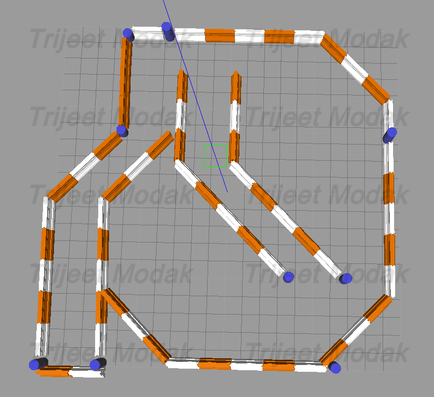
\includegraphics[scale=0.5]{imgs/map-jackal-race.png}
    \centering
    \caption{world map used for localization in the simulated environment}
    \label{fig:map-jackal-race}
\end{figure}

ROS's AMCL package and Navigation Stack package are used incorporate localization and navigation features into the bot models.

\subsection{Udacity Bot - A Benchmark Model}
\subsubsection{Model Design}
The provided benchmark robot, named as udacity bot, was developed by creating a Unified Robot Description file (UDRF) using the design description provided by Udacity in the classroom course. The size and geometry as well as the physical configuration of the robot such as inertial and collision parameters are specified using the UDRF file. The details are tabulated in table \ref{table:desc-udacity-bot} and the corresponding visuals are shown in Fig. \ref{fig:udacity-bot}.

\begin{table}[h]
\renewcommand{\arraystretch}{1.5}
\centering
\begin{tabular}{|l|c|c|}
\hline
\textit{\textbf{Component}} & \textit{\textbf{Geometry}}    & \textit{\textbf{Mass}} \\ \hline
\textit{Base/Chassis}       & Box (l = 0.4, w = 0.2, h=0.1) & 15.0                   \\ \hline
\textit{Front/Back Castor}  & Sphere (r = 0.1)              & (incl. in chassis)     \\ \hline
\textit{Left/Right  Wheels} & Cylinder (r = 0.1, l = 0.05)  & 5.0                    \\ \hline
\textit{Camera}             & Box (0.05 ✕ 0.05 ✕ 0.05)      & 0.1                    \\ \hline
\textit{Hokuyo Laser}       & Box (0.01 ✕ 0.01 ✕ 0.01       & 0.1                    \\ \hline
\end{tabular}
\vspace{5pt}
\caption{Udacity Bot Description}
\label{table:desc-udacity-bot}
\end{table}

\begin{figure}[h]
    \centering
    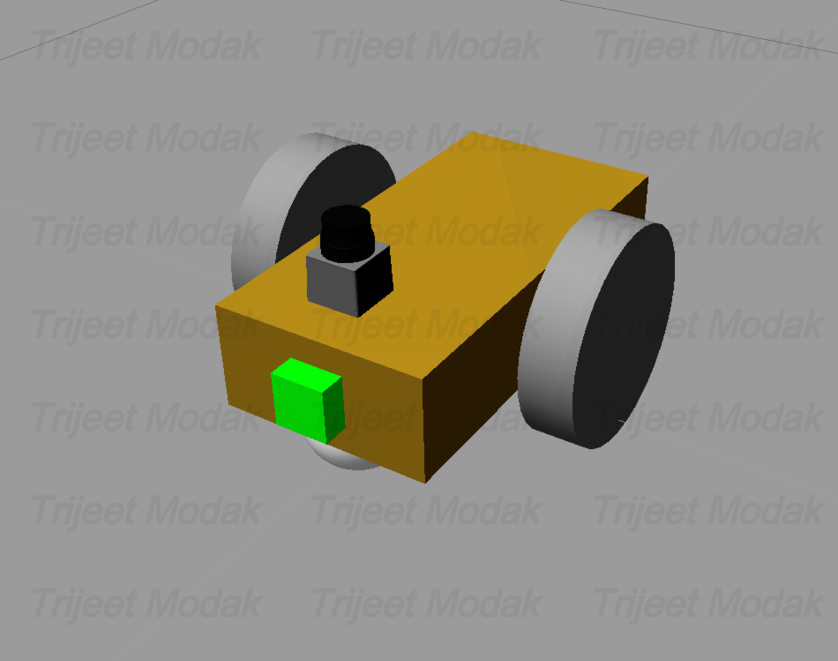
\includegraphics[scale=0.225]{imgs/udacity-bot.png}
    \centering
    \caption{Udacity-Bot design}
    \label{fig:udacity-bot}
\end{figure}


\subsubsection{Parameters}
To obtain accurate localization results, several parameters are added and tuned iteratively. The most prominent parameters were the max particles and min particles which were set to 100 and 10 respectively. While increasing the values of these parameters increases accuracy, it would add extra overhead to the computation, making the process slower. The other parameters that were tuned iteratively are transform tolerance, inflation radius, and obstacle range. Apart from these parameters, a few parameters like update\_min\_d  and update\_min\_a were added to optimize the computation required for the robot movement.

The transform tolerance is the time with which to postdate the transform that is published, to indicate that this transform is valid in future. This was a key parameter affecting the stability of the model that has to be modified to be larger than the update frequency which was set to 5 Hz.

The inflation radius is an important parameter that affects the costmap while detecting obstacles and their distance related to the robot. 

\begin{table}[h]
\renewcommand{\arraystretch}{1.5}
\centering
\begin{tabular}{|l|l|}
\hline
\textit{\textbf{Parameter}} & \textit{\textbf{Value Used}} \\ \hline
\textit{min\_particles}     & 10                           \\ \hline
\textit{max\_particles}     & 100                          \\ \hline
\textit{update\_min\_d}     & 0.01                         \\ \hline
\textit{update\_min\_a}     & 0.01                         \\ \hline
\end{tabular}
\vspace{5pt}
\caption{Udacity Bot AMCL Parameters}
\label{table:amcl-params-udacity-bot}
\end{table}

\begin{table}[h]
\renewcommand{\arraystretch}{1.5}
\centering
\begin{tabular}{|l|l|}
\hline
\textit{\textbf{Parameter}}   & \textit{\textbf{Value Used}} \\ \hline
\textit{obstacle\_range}      & 5.25                         \\ \hline
\textit{raytrace\_range}      & 7.75                         \\ \hline
\textit{transform\_tolerance} & 0.2                          \\ \hline
\textit{inflation\_radius}    & 0.5                          \\ \hline
\end{tabular}
\vspace{5pt}
\caption{Udacity Bot Costmap Parameters}
\label{table:cost-params-udacity-bot}
\end{table}

\begin{table}[h]
\renewcommand{\arraystretch}{1.5}
\centering
\begin{tabular}{|l|l|}
\hline
\textit{\textbf{Parameter}}         & \textit{\textbf{Values Used}} \\ \hline
\textit{sim\_time}                  & 1.0                           \\ \hline
\textit{pdist\_scale}               & 0.5                           \\ \hline
\textit{yaw\_goal\_tolerance}       & 0.025                         \\ \hline
\textit{xy\_goal\_tolerance}        & 0.05                          \\ \hline
\textit{controller\_frequency}      & 5                             \\ \hline
\textit{acc\_lim\_x}                & 3                             \\ \hline
\textit{acc\_lim\_y}                & 3                             \\ \hline
\textit{acc\_lim\_theta}            & 3                             \\ \hline
\textit{max\_vel\_x}                & 0.4                           \\ \hline
\textit{min\_vel\_x}                & 0.05                          \\ \hline
\textit{max\_vel\_theta}            & 1.0                           \\ \hline
\textit{min\_vel\_theta}            & -1.0                          \\ \hline
\textit{min\_in\_place\_vel\_theta} & 0.2                           \\ \hline
\end{tabular}
\vspace{5pt}
\caption{Udacity Bot Base-Local Parameters}
\label{table:base-local-params-udacity-bot}
\end{table}


\subsection{RoboND Bot}
\subsubsection{Model Design}
The personal named robot, RoboND robot, was developed by creating a new UDRF file all within the same udacity package with remapped publishers and subscribers. In this file the size and geometry of the robot is designated and set to have physical configuration such as inertial and collision parameters. The chassis of the bot consists three parts, a cylinder of radius 0.15 and length of 0.1 at the base, a box with dimension 0.1 x 0.1 x 0.2 in the middle and a sphere of radius 0.1 at the top. A sphere shaped castor of radius 0.3125 is attached to the front to provide balance to the robot. The left and right wheels are of cylindrical shape with radius 0.03 and length 0.02, are connected to the chassis via continuous joints, meaning they are free to rotate along the joint axis. The robot is also equipped with a box shaped camera and a Hokuyo laser scanner.(Refer to TABLE \ref{table:desc-robond-bot} for detailed descriptions and Fig. \ref{fig:robond-bot} for visuals)

\begin{table}[h]
\renewcommand{\arraystretch}{1.5}
\centering
\begin{tabular}{|l|c|c|}
\hline
\textit{\textbf{Component}}    & \textit{\textbf{Geometry}}    & \textit{\textbf{Mass}}                  \\ \hline
\textit{Base/Chassis}          & Composite                     & 25.0                                    \\ \hline
\textit{Base/Chassis - Part 1} & Cylinder (r = 0.15, l =0.1)   & \multicolumn{1}{l|}{(incl. in chassis)} \\ \hline
\textit{Base/Chassis - Part 2} & Box (0.1 ✕ 0.1 ✕ 0.2)         & \multicolumn{1}{l|}{(incl. in chassis)} \\ \hline
\textit{Base/Chassis - Part 3} & Sphere (r = 0.1)              & \multicolumn{1}{l|}{(incl. in chassis)} \\ \hline
\textit{Front Castor}          & Sphere (r = 0.3125)           & (incl. in chassis)                      \\ \hline
\textit{Left/Right  Wheels}    & Cylinder (r = 0.03, l = 0.02) & 10.0                                    \\ \hline
\textit{Camera}                & Box (0.05 ✕ 0.05 ✕ 0.05)      & 0.1                                     \\ \hline
\textit{Hokuyo Laser}          & Box (0.01 ✕ 0.01 ✕ 0.01       & 0.1                                     \\ \hline
\end{tabular}
\vspace{5pt}
\caption{RoboND Bot Description}
\label{table:desc-robond-bot}
\end{table}

\begin{figure}[h]
    \centering
    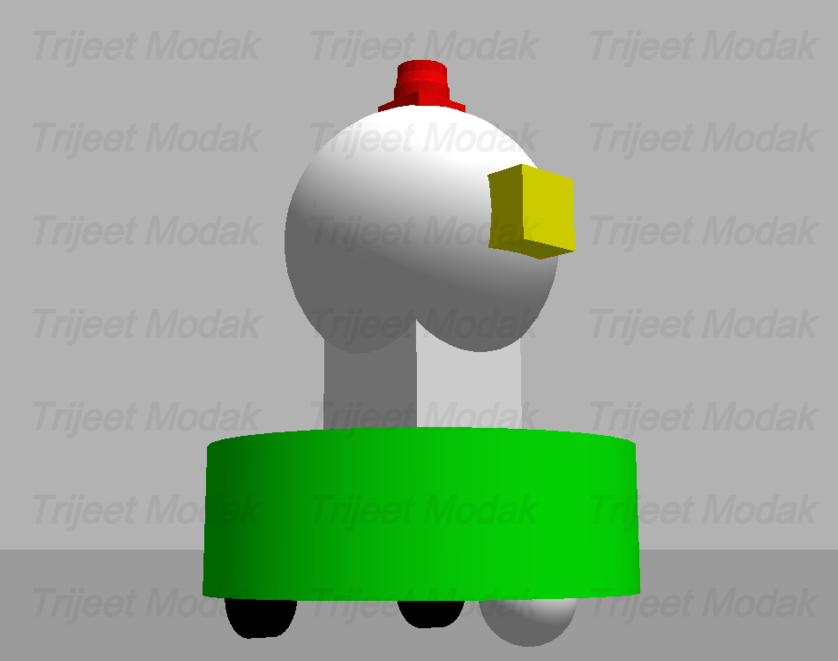
\includegraphics[scale=0.225]{imgs/robond-bot.png}
    \centering
    \caption{RoboND-Bot description}
    \label{fig:robond-bot}
\end{figure}


\subsubsection{Parameters}
For the RoboND, most of the parameters of the udacity bot had to be modified to successfully solve the localization problem as the body and the shape of the RoboND bot is completely different from the udacity bot. Since the chassis of the robot consists of three parts, the mass of the robot was increased to 25 to make it more stable. Due to increased mass, the magnitude of maximum and minimum angular velocity had to be increased to allow the robot to steer properly. The costmap parameters were also changed to accommodate the changes in the robot design.(See TABLE \ref{table:amcl-params-robond-bot}, TABLE \ref{table:cost-params-robond-bot} and TABLE \ref{table:base-local-params-robond-bot} for detailed specifications.)
\begin{table}[h]
\renewcommand{\arraystretch}{1.5}
\centering
\begin{tabular}{|l|l|}
\hline
\textit{\textbf{Parameter}} & \textit{\textbf{Value Used}} \\ \hline
\textit{min\_particles}     & 10                           \\ \hline
\textit{max\_particles}     & 150                          \\ \hline
\textit{update\_min\_d}     & 0.005                        \\ \hline
\textit{update\_min\_a}     & 0.005                        \\ \hline
\end{tabular}
\vspace{5pt}
\caption{RoboND Bot AMCL Parameters}
\label{table:amcl-params-robond-bot}
\end{table}

\begin{table}[h]
\renewcommand{\arraystretch}{1.5}
\centering
\begin{tabular}{|l|l|}
\hline
\textit{\textbf{Parameter}}   & \textit{\textbf{Value Used}} \\ \hline
\textit{obstacle\_range}      & 4.5                         \\ \hline
\textit{raytrace\_range}      & 10.0                         \\ \hline
\textit{transform\_tolerance} & 0.2                          \\ \hline
\textit{inflation\_radius}    & 0.55                          \\ \hline
\end{tabular}
\vspace{5pt}
\caption{RoboND Bot Costmap Parameters}
\label{table:cost-params-robond-bot}
\end{table}

\begin{table}[h]
\renewcommand{\arraystretch}{1.5}
\centering
\begin{tabular}{|l|l|}
\hline
\textit{\textbf{Parameter}}         & \textit{\textbf{Values Used}} \\ \hline
\textit{sim\_time}                  & 1.0                           \\ \hline
\textit{pdist\_scale}               & 0.25                           \\ \hline
\textit{yaw\_goal\_tolerance}       & 0.05                         \\ \hline
\textit{xy\_goal\_tolerance}        & 0.05                          \\ \hline
\textit{controller\_frequency}      & 5                             \\ \hline
\textit{acc\_lim\_x}                & 2                             \\ \hline
\textit{acc\_lim\_y}                & 2                             \\ \hline
\textit{acc\_lim\_theta}            & 2                             \\ \hline
\textit{max\_vel\_x}                & 1.0                           \\ \hline
\textit{min\_vel\_x}                & 0.05                          \\ \hline
\textit{max\_vel\_theta}            & 1.5                           \\ \hline
\textit{min\_vel\_theta}            & -1.5                          \\ \hline
\textit{min\_in\_place\_vel\_theta} & 1.0                           \\ \hline
\end{tabular}
\vspace{5pt}
\caption{RoboND Bot Base-Local Parameters}
\label{table:base-local-params-robond-bot}
\end{table}
 
\section{Results}
\subsection{Localization results}
\subsubsection{Udacity-Bot}
The bot quickly localized itself and made a smooth traversal from its initial position towards the goal. Since the end goal yaw tolerance was set to very low, it took a while to adjust its orientation before coming to a full stop at the goal location.

\begin{figure}[h]
    \centering
    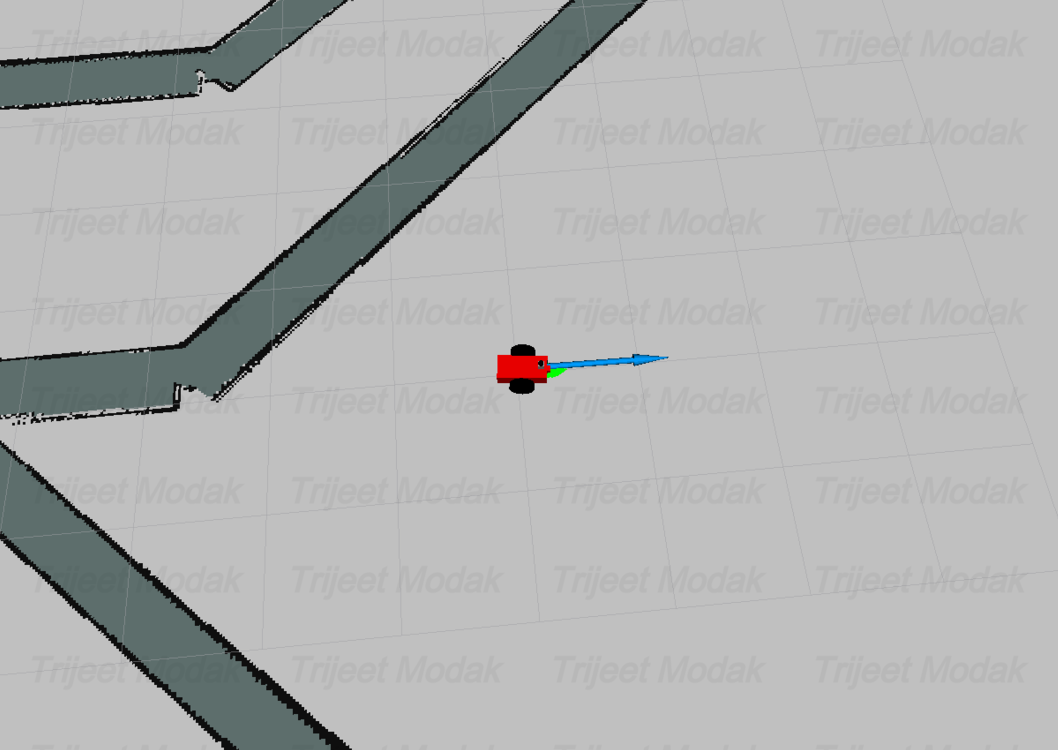
\includegraphics[scale=0.225]{imgs/udacity-bot-goal.png}
    \centering
    \caption{Udacity-Bot reached the goal location}
    \label{fig:udacity-bot-goal}
\end{figure}

\begin{figure}[h]
    \centering
    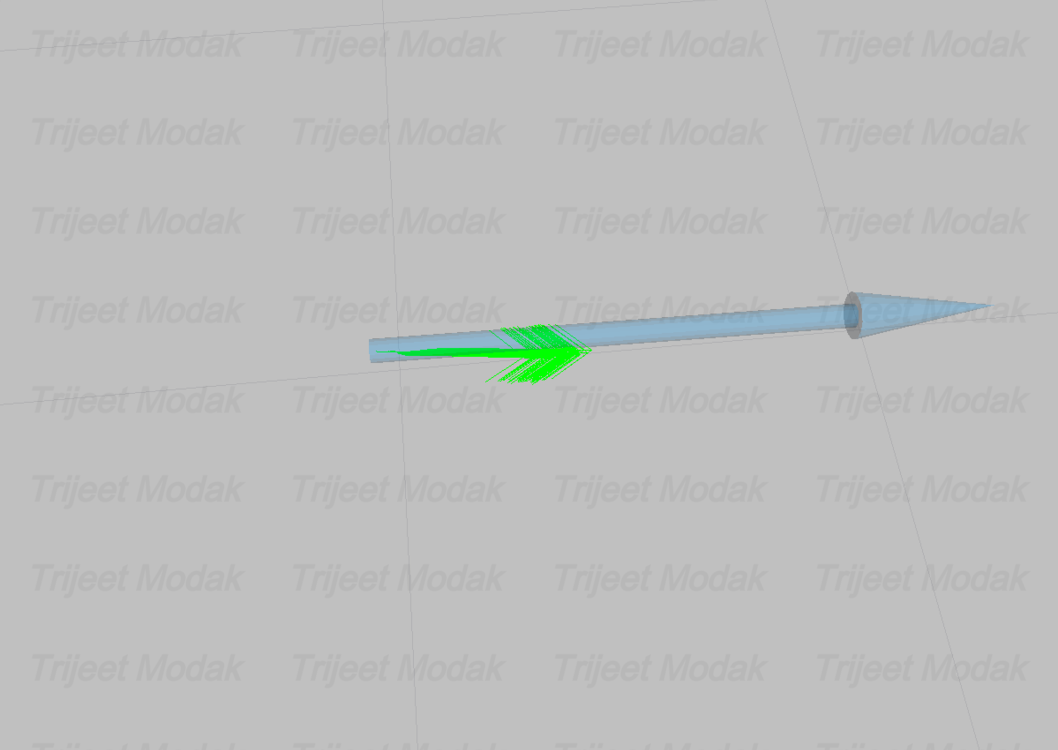
\includegraphics[scale=0.225]{imgs/udacity-goal-orientation.png}
    \centering
    \caption{A closer view of the goal location/orientation (blue) vs final Udacity-Bot position/orientation (green)}
    \label{fig:udacity-goal-orientation}
\end{figure}


\subsubsection{RoboND-Bot}
After quite a long process of parameter tuning, the bot finally travelled smoothly from the initial position to the goal position. Initially, since the bot wheels are too small, the bot moved in a very unstable way. Increasing the mass increased its stability, but it caused the bot to be unable to quickly adapt to direction changes. Finally the problem was solved by increasing the angular velocities and decreasing the acceleration rates.

\begin{figure}[h]
    \centering
    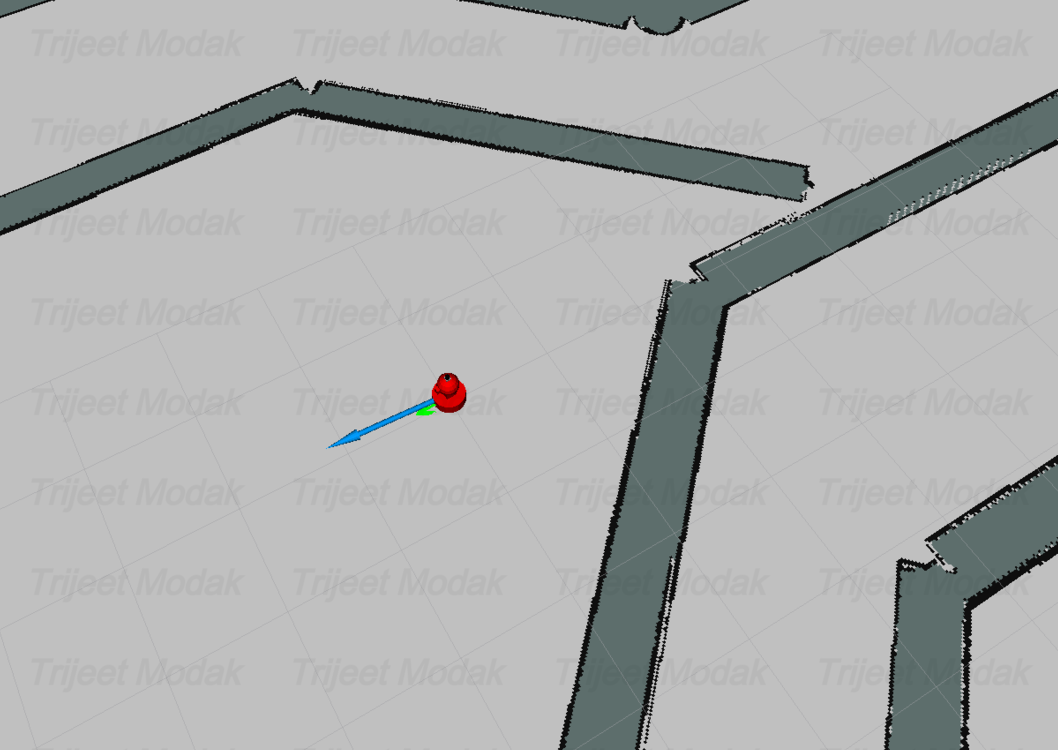
\includegraphics[scale=0.225]{imgs/robond-bot-goal.png}
    \centering
    \caption{RoboND-Bot reached the goal location}
    \label{fig:robond-bot-goal}
\end{figure}



\begin{figure}[h]
    \centering
    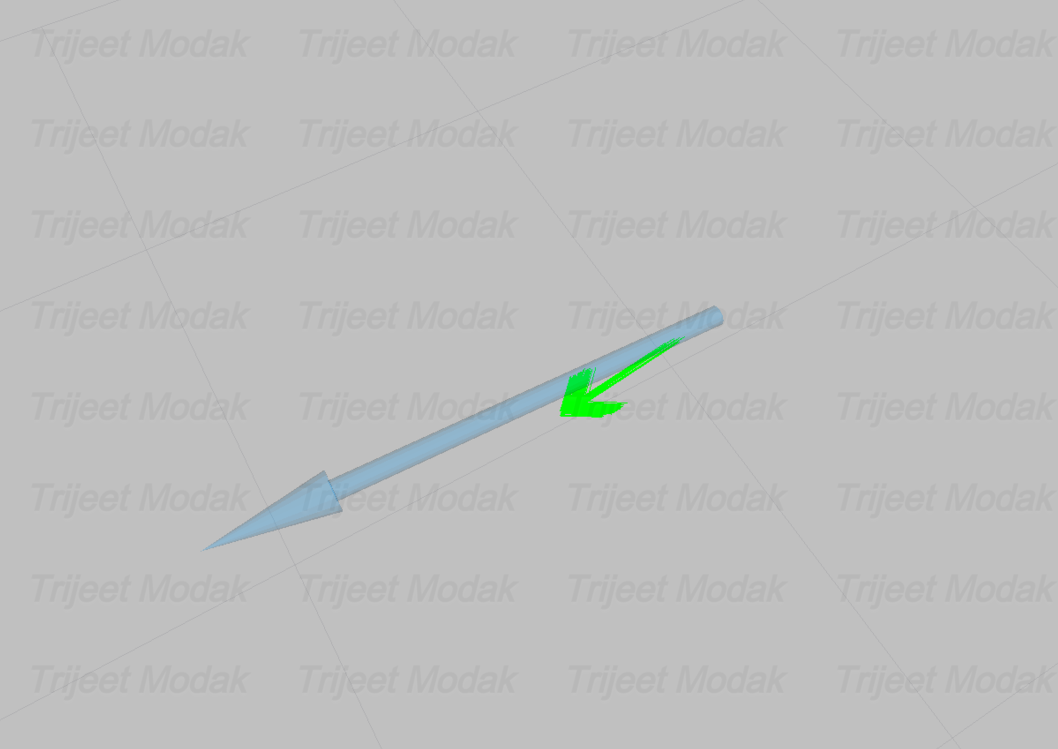
\includegraphics[scale=0.225]{imgs/robond-goal-orientation.png}
    \centering
    \caption{A closer view of the goal location/orientation (blue) vs final RoboND-Bot position/orientation (green)}
    \label{fig:robond-goal-orientation}
\end{figure}

\subsection{Technical Comparison}
Given the design and parameters difference between two mobile robots, the turning and steering performance differs slightly. The udacity bot could follow the path well while the RoboND bot took few deviations in the curve, making the udacity bot performance slightly better. Both the bots were able move smoothly, avoiding obstacles, localizing properly and reaching the destination under 2 minutes.

\section{Discussion}
Overall, the udacity benchmark model performed much better than RoboND bot, possibly due to the optimum physical configuration that allows it to travel faster through the map. However, both the robots were able to perform well throughout their trajectory. Both models reached the designated goal successfully while localizing themselves on the map and avoiding obstacles.

As for the kidnapped vehicle problem, it can be understood that both the bot models can solve the scenario. Although the required number of particles to solve it will be much greater than the current scenario as the initial location of the robot is unknown. Localizing it would take more time and the computation will depend on the size of the map.

Localization is an important module in robotics and are used for robots moving in warehouses to self driving cars. Although MCL/AMCL packages are ideal candidates for localizing in indoor environments, they are computational expensive and requires lot of effort in tuning the parameters.

\section{Conclusion/ Future Work}
It can be concluded that AMCL is a powerful tool to solve localization problem for robots in indoor environments. The fact that it is very easy to implement and the immense community support for its package makes it the first choice of algorithm for developing autonomous bots. In future work, implementing AMCL for 3D localization would be the next step. This could be used for localizing drones and arm actuators that needs end-effector location and  orientation to reach the desired goal.

\bibliography{bib}
\bibliographystyle{ieeetr}

\end{document}